\problemname{Magical Mystery Knight's Tour}

A knight's tour on a rectangular board of $n$ rows and $m$ columns of squares (traditionally 8-by-8) 
is a labelling of the squares by integers $1$ through $n * m$ so that label $n+1$ is a knight's move from label $n$.
That is, $2$ squares horizontally and $1$ square vertically or $1$ square horizontally and $2$ squares
vertically. The image below shows an 8-by-8 knight's tour.

\begin{figure}[!h]
\begin{center}
    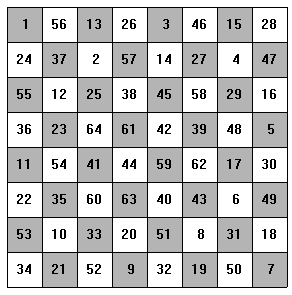
\includegraphics[width=.35\textwidth]{knight-001.png}
\end{center}
\end{figure}

A knight's tour (on a square board) is (\emph{semi-})magical if the sum of the values in each row and column
is the same (for the 8-by-8 case the sum would be $260$). For this problem, you will be given a
sequence of semi-magical 8-by-8 knight's tours with many of the labels removed (see the image
below). Write a program to fill in the missing labels so the knight's tour is \emph{semi-}magical.

\begin{figure}[!h]
\begin{center}
    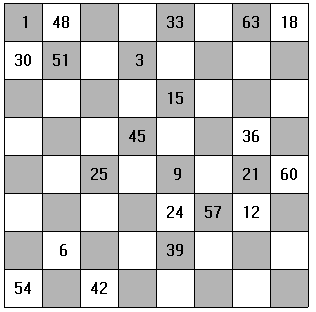
\includegraphics[width=.35\textwidth]{knight-002.png}
\end{center}
\end{figure}

\section*{Input}

The input contains a single data set consisting of $8$ lines of
input.  Each line contains $8$ integers
separated by spaces giving the labels for the corresponding row. If the
label value is $-1$, the label has been removed and your program is to
find the correct value to put in that place.
There will be at most $45$ removed labels with the value $-1$.
You may assume that the starting point of the tour (labeled $1$) was
not removed and thus appears in the input.

\section*{Output}

Output $8$ lines containing $8$ integers each, separated by spaces, filling in the removed
values to give a complete semi-magical knight's tour which includes the positive labels from the input.
There may be multiple correct answers.  Your result will be graded correct if it is a semi-magical
knight's tour and the positive labels from the input are in the same square in your answer.

\emph{Note:} Your output does not have to be lined up as shown in the Sample Output. Just make
sure that each of the $8$ lines of output has at least one space between each value on the line.

